\documentclass[../main.tex]{subfiles}
\graphicspath{{\subfix{../images/}}} % Images path

\begin{document}

\section{Visual Vocabulary Construction}\label{sec:visual-vocabulary-construction}

The process of building a visual vocabulary can be split in two main steps: 

\begin{enumerate}
  \item \textbf{Feature extraction}: sampling of SIFT descriptors from train images.
  \item \textbf{Clustering}: grouping of the extracted descriptors into $K$ clusters.
\end{enumerate}

\subsection{Feature Extraction}\label{subsec:feature-extraction}

The first step involves the extraction of local features from the images in the
training set. In this case, SIFT descriptors have been used as features, and they
have been extracted following two different approaches:

\begin{enumerate}
  \item Using the \bft{SIFT detector}: the SIFT detector is used to detect keypoints in the images and the corresponding SIFT descriptors are computed on these keypoints.
  \item Sampling on a \bft{dense regular grid}: following the approach adopted
	  by \itt{Lazebnik et al.}~\cite{lazebnik}, SIFT descriptors can also be
	  computed from keypoints sampled on a regular dense grid over each image.
	  Following the approach of the paper, a regular grid with spacing of $8$ pixels between each keypoint has been used.
\end{enumerate}

% As highlighted by \itt{Lazebnik et al.} [TOOD: add reference] reporting the original evaluation from \itt{Fei-Fei and Perona} [TOOD: add reference], sampling descriptors from a regular grid should intuitively work better from scene classification tasks, as this method allows to capture uniform regions such as sky, calm water, or road surfaces.\\
Both sampling methods have been tested and compared, with the results shown in
later section~\ref{sec:results}. 
For the first approach, the SIFT detector has
been initialized to retain only the best $500$ features in each image, resulting in a total of $\num{593006}$ keypoints, while for the second approach $\num{1482434}$ keypoints have been collected.\\
Notice that with both approaches the exact number of keypoints extracted in each
image can change from one image to another.
In the first case, this is due to
the content of the images, i.e.\ the actual number of features that can be
detected by the SIFT detector.
In the second case instead, this is due to the different sizes and aspect ratios of the images. 
Figure~\ref{fig:keypoints-example} shows an example of this phenomenon, where a
different number of keypoints has been detected by the SIFT detector in two
different images, while Appendix~\ref{app:keypoints-distribution} shows the
distribution descriptors sampled from the train set with the two methods.

\begin{figure}[H]
  \centering
  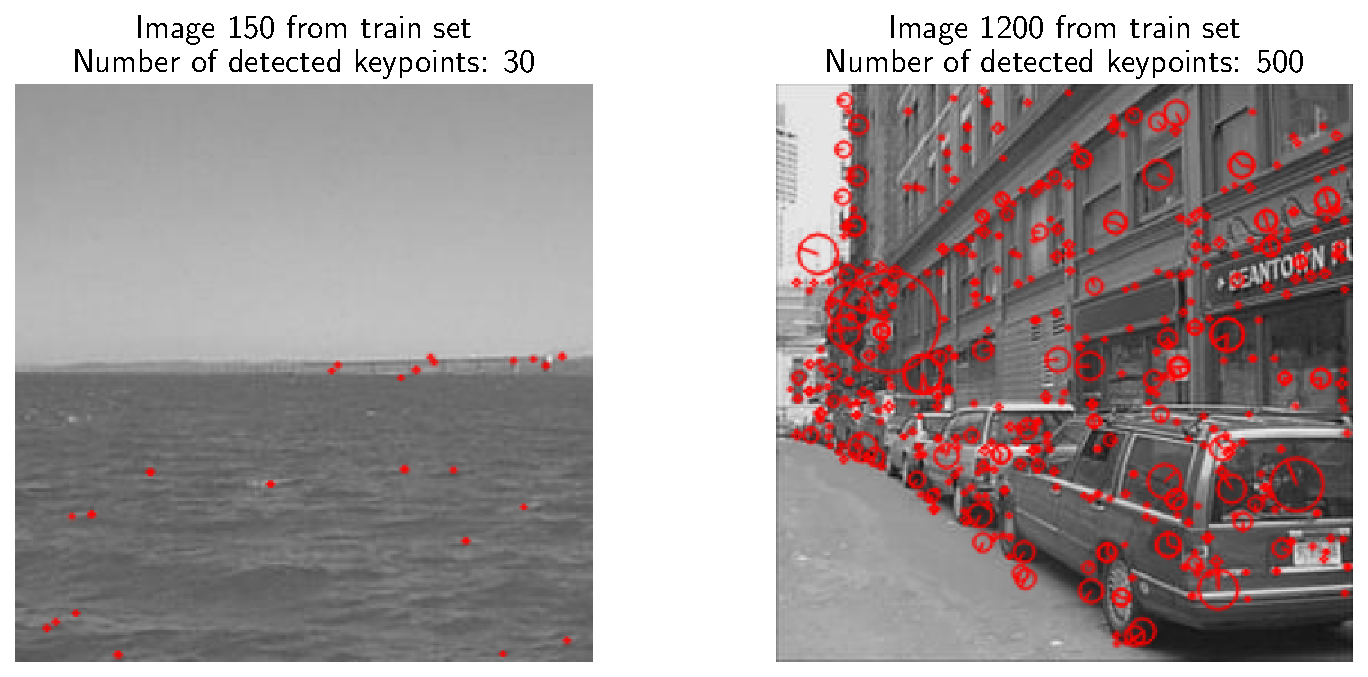
\includegraphics[width=0.9\textwidth]{keypoints.pdf}
  \caption{Example of keypoints detection with the SIFT detector. In the left
  side image only $30$ keypoints were detected, while in the right side one all
the desired $500$ keypoints were found.}
  \label{fig:keypoints-example}
\end{figure}


\subsection{Clustering}\label{subsec:clustering}

Following feature extraction, clustering has been performed on a random subset
of extracted SIFT descriptors to build the visual vocabulary. Hence, the
resulting centroids, representing the visual words of the vocabulary, are
$128$-dimensional vectors.\\
The size of the subset has been chosen to maintain about the same ratio between the
total number of descriptors and the number of descriptors used for
clustering in the two feature extraction methods. Hence, this has been set to
$\num{10000}$ for descriptors sampled using the SIFT detector and to
$\num{25000}$ for descriptors sampled on a regular grid.\\
Clustering has then been performed using the \itt{k-means} algorithm to group
descriptors into $K$ clusters, where $K$ becomes the size of the visual
vocabulary. The number of clusters is an hyperparameter of the
clustering process which has to be chosen. An analysis of the average silhouette
score~\cite{silhouette} has been performed for values of $K$ ranging from $50$
to $1000$ with the results shown in figure~\ref{fig:silhouette-score}.
Ultimately, the value of $K=400$ has been chosen as a good trade-off between the
quality of the clustering and the overall computational cost of the clustering process.
Moreover, the choice is also motivated by the final results obtained in
Section~\ref{sec:results} and by the fact that, given the objectives of
this project, this value allows for a direct comparison with the results
reported by \itt{Lazebnik et al.}~\cite{lazebnik}, where the same vocabulary
size was used.
\begin{figure}[htb]
  \centering
  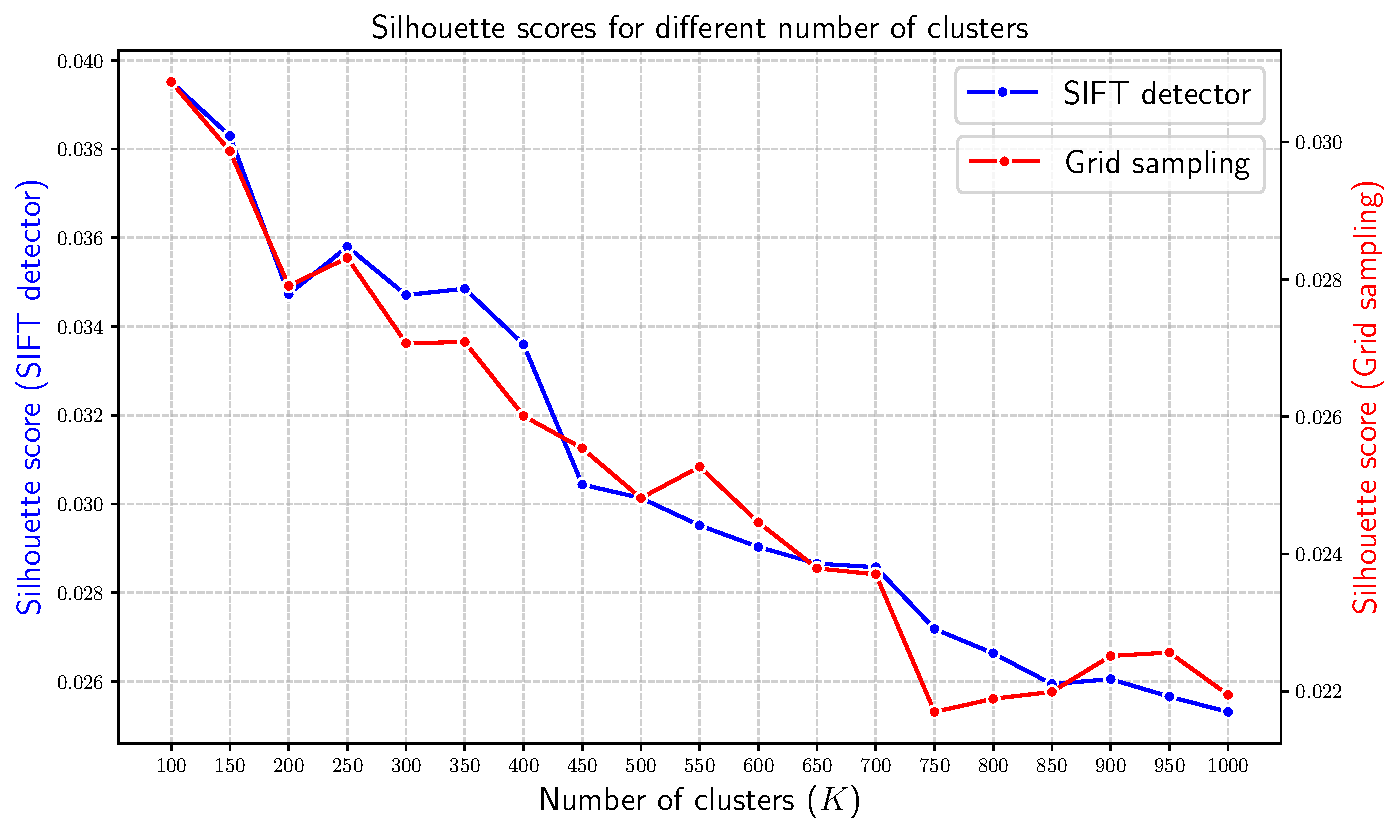
\includegraphics[width=0.9\textwidth]{silhouette_scores_comparison.pdf}
  \caption{Silhouette scores resulting from
  clustering SIFT descriptors sampled using the SIFT detector (\itt{blue})
and on a regular grid (\itt{red}). As expected, the value decreases with the
increase of $K$. Noticeable decreases occur after $K\approx400$ and $K\approx700$.}
  \label{fig:silhouette-score}
\end{figure}

\end{document}

